\section{ĐỘNG HỌC THUẬN}
\subsection{Mô phỏng hình dạng Robot}
\subsubsection{Xác định các thông số và lập bảng DH}

Để có thể mô phỏng lại hình dạng robot, ta cần biết được vị trí của các khớp
trong hệ toạ độ XYZ từ đó nối các điểm các khớp lại ta sẽ được hình dạng cơ bản của robot Articulated arm trong không gian.

Articulated arm là robot 3 bậc tự do, do đó, để có được vị trí của các khớp so
với base, ta cần tính các ma trận biến đổi thuận nhất của các khớp so với base, từ
đó lấy ra thông số vị trí và hướng của các khớp.

\begin{figure}[H]
	\centering
	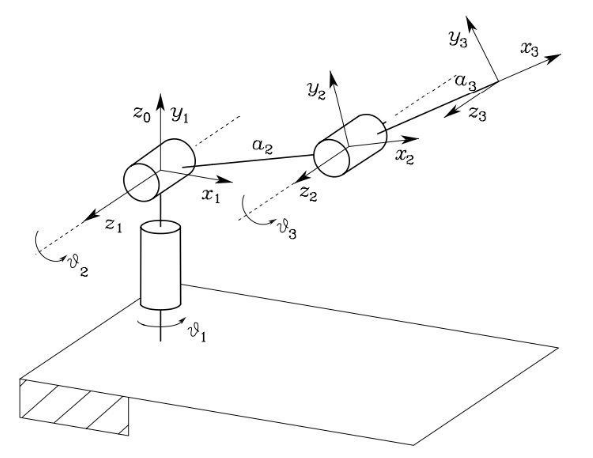
\includegraphics[width=0.8\linewidth]{Images/arti_arm.png}
	\caption{Articulated Arm}
	\label{fig:enter-label3}
\end{figure}

Đầu tiên ta cần thiết lập bảng DH, từ đó có thể thấy, các biến của robot
Articulated arm là $\theta_{1}$ , $\theta_{2}$ và $\theta_{3}$

\begin{center}
	\begin{tabular}{|m{2cm}|m{2cm}|m{2cm}|m{2cm}|m{2cm}|} 
		\hline
		Link & $a_{i}$ & $\alpha_{i}$ & $d_{i}$ & $\theta_{i}$\\ [0.5ex] 
		\hline
		1 & 0 & $\pi/2$ & $d_{1}$ & $\theta_{1}^{*}$\\ 
		\hline
		2 & $a_{2}$ & 0 & 0 & $\theta_{2}^{*}$\\
		\hline
		3 & $a_{3}$ & 0 & 0 & $\theta_{3}^{*}$\\ [0.5ex] 
		\hline
	\end{tabular}
\end{center}

Sau khi có bảng DH, ta viết các hàm để tính toán ma trận biến đổi thuần nhất với input là các giá trị lấy từ ma trận DH.

\vspace{0.5cm}
\begin{lstlisting}[language=python]
	# % Link | d   | theta        |   a   | alpha
	# % 1      d1    theta_1          0      90
	# % 2      0     theta_2         a2       0
	# % 3      0     theta_3         a3       0 
	d = np.array([100, 0, 0])
	a = np.array([0, 100, 100])
	alpha = np.array([pi/2, 0, 0])
	theta = np.array([0, 0, 0])
	offsetTheta = np.array([0, 0, 0])
	
	# Calculate DH matrix function
	def DH_Matrix(d, theta, a, alpha):
	c = cos(theta)
	s = sin(theta)
	ca = cos(alpha)
	sa = sin(alpha)
	return np.array([
	[c, -ca*s, sa*s, a*c],
	[s, c*ca, -sa*c, a*s],
	[0, sa, ca, d],
	[0, 0, 0, 1],
	])
	
	# Calculate Tranpose matrix T0, T1, T2, T3 function
	def updateTranposeMatrix():
	T0 = np.eye(4)
	T1 = np.dot(T0, DH_Matrix(d[0], theta[0]+offsetTheta[0], a[0], alpha[0]))
	T2 = np.dot(T1, DH_Matrix(d[1], theta[1]+offsetTheta[1], a[1], alpha[1]))
	T3 = np.dot(T2, DH_Matrix(d[2], theta[2]+offsetTheta[2], a[2], alpha[2]))
	return [T0, T1, T2, T3]
\end{lstlisting}

\subsubsection{Xây dựng môi trường giả lập Robot}

Vì ở bài tập lớn này ta không sử dụng thư viên 3D mà sử dụng thư viện vẽ 2D là \textit{Pygame} để vẽ robot nên ta phải dùng phép chiếu hình 3D lên màn hình 2D.

Ta sẽ tạo các biến $angleX$, $angleY$ và $angleZ$ để lưu lại các góc xoay lần lượt theo trục $x$, $y$ và $z$ (\textit{hay còn gọi là góc Roll-Pitch-Yaw}) của tọa độ chuẩn môi trường giả lập robot so với góc nhìn của chúng ta, các góc trên sẽ thay đổi dựa vào tương tác của người dùng trên UI hoặc qua bàn phím, chuột, ... . Ta viết được hàm chiếu 2D đơn giản với input là 1 điểm trong hệ $Oxyz$ sang $Oxy$ (\textit{Vì mô phỏng robot đơn giản chỉ có các điểm và đường nên ta có thể bỏ qua z}).

\vspace{0.5cm}
\begin{lstlisting}[language=python]
	scale = 1.5
	angleX = -3*pi/4
	angleY = 0
	angleZ = -pi/4
	
	def projective(pos):
	pos = pos.reshape((3, 1))
	rotation_z = np.array([
	[cos(angleZ), -sin(angleZ), 0],
	[sin(angleZ), cos(angleZ), 0],
	[0, 0, -1],
	])
	rotation_y = np.array([
	[cos(angleY), 0, sin(angleY)],
	[0, 1, 0],
	[-sin(angleY), 0, cos(angleY)],
	])
	rotation_x = np.array([
	[1, 0, 0],
	[0, cos(angleX), -sin(angleX)],
	[0, sin(angleX), cos(angleX)],
	])
	pos = np.dot(rotation_z, pos)
	pos = np.dot(rotation_y, pos)
	pos = np.dot(rotation_x, pos)
	x = pos[0][0]
	y = pos[1][0]
	z = pos[2][0]
	xx = int(x * scale) + circle_pos[0]
	yy = int(y * scale) + circle_pos[1]
	return (xx, yy)
\end{lstlisting}

Tiếp tục ta sẽ viết các hàm vẽ các điểm, đường, polygon và trục tọa độ $Oxyz$ để hỗ trợ vẽ robot sau này.

\vspace{0.5cm}
\begin{lstlisting}[language=python]
	def drawCoor(screen, poso, posx, posy, posz):
	o = projective(poso)
	x = projective(posx)
	y = projective(posy)
	z = projective(posz)
	pygame.draw.circle(screen, BLACK, o, 3)
	pygame.draw.line(screen, RED, o, x, width=2)
	pygame.draw.line(screen, BLUE, o, y, width=2)
	pygame.draw.line(screen, GREEN, o, z, width=2)
	def drawCircle(screen, pos, color=RED, radius=1, width=0):
	pos = projective(pos)
	pygame.draw.circle(screen, color, pos, radius, width)
	def drawLine(screen, posx, posy, color=ORANGE, width=1):
	x = projective(posx)
	y = projective(posy)
	pygame.draw.line(screen, color, x, y, width)
	def drawPolygon(screen, posArray, color):
	pygame.draw.polygon(screen, color, [projective(p) for p in posArray], 0)
\end{lstlisting}

\subsubsection{Vẽ Robot}

Dựa và vị trí gốc (base) của robot và các ma trận biến đổi thuần nhất ta tính toán ra được các vị trí của các khớp xoay (joint) trong không gian và dùng hàm vẽ có được ở trên để vẽ ra được robot, các trục tọa độ và cả mặt đất bên dưới robot.

\vspace{0.5cm}
\begin{lstlisting}[language=python]
	def drawMachine(opacity, T):
	s = pygame.Surface((WIDTH,HEIGHT), pygame.SRCALPHA)
	ground = np.array([[-100, -100, 0], [-100, 100, 0], [100, 100, 0], [100, -100, 0]])
	drawPolygon(s, ground ,(0,0,0,opacity))     
	drawCircle(s, DHtranspose(baseO, T[0]), color=(255,0,0,opacity), radius=5)
	drawCircle(s, DHtranspose(baseO, T[1]), color=(255,0,0,opacity), radius=5)
	drawCircle(s, DHtranspose(baseO, T[2]), color=(255,0,0,opacity), radius=5)
	drawCircle(s, DHtranspose(baseO, T[3]), color=(255,0,0,opacity), radius=5)
	drawLine(s, DHtranspose(baseO, T[0]), DHtranspose(baseO, T[1]), color=(230,0,180,opacity), width=5)
	drawLine(s, DHtranspose(baseO, T[1]), DHtranspose(baseO, T[2]), color=(230,0,180,opacity), width=5)
	drawLine(s, DHtranspose(baseO, T[2]), DHtranspose(baseO, T[3]), color=(230,0,180,opacity), width=5)
	screen.blit(s, (0,0))
\end{lstlisting}

\begin{figure}[H]
	\centering
	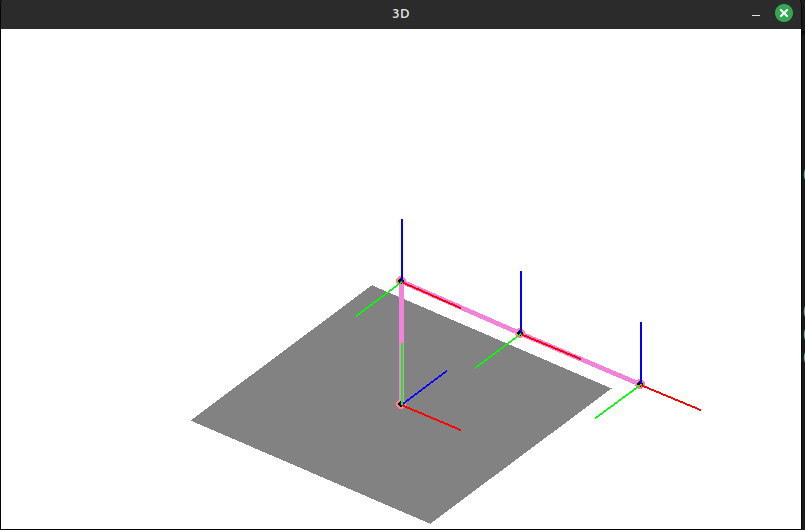
\includegraphics[width=1\linewidth]{Images/draw_bot.png}
	\caption{Vẽ robot}
	\label{fig:enter-label4}
\end{figure}

\subsection{Xây dựng UI và Animation cho bài toán động lực thuận}
\subsubsection{Giao điện người dùng UI}

Sử dụng thư viên \textit{Tkinter} để xây dựng giao diện người dùng. Xây dựng một cửa sổ đẻ tùy chỉnh các thông số đẽ vẽ robot và in các thông số cơ bản của robot như vị trí và góc xoay RPY của Tool (\textit{End Effector}).

\vspace{0.5cm}
\begin{lstlisting}[language=python]
	def calRPY(T):
	pitch = atan2(-T[2][0], sqrt(T[2][1]**2 + T[2][2]**2))
	if pitch == pi/2:
	yaw = 0
	rall = atan2(T[0][1], T[1][1])
	elif pitch == -pi/2:
	yaw = 0
	rall = -atan2(T[0][1], T[1][1])
	else:
	yaw = atan2(T[1][0]/cos(pitch), T[0][0]/cos(pitch))
	rall = atan2(T[2][1]/cos(pitch), T[2][2]/cos(pitch))
	return str(round(rall*180/pi, 3)) + " | " + str(round(pitch*180/pi, 3)) + " | " + str(round(yaw*180/pi, 3))
\end{lstlisting}

\begin{figure}[H]
	\centering
	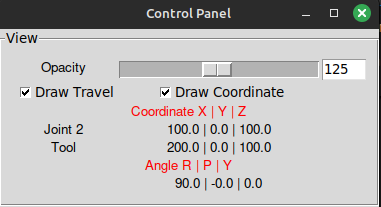
\includegraphics[width=1\linewidth]{Images/view_ui.png}
	\caption{Giao diện View}
	\label{fig:enter-label5}
\end{figure}

Xây dựng giao diện để người dùng nhập các góc $\theta_{1}$ , $\theta_{2}$ và $\theta_{3}$, sau khi bấm nút \textit{Execute} robot sẽ tiến hành di chuyển theo các góc $\theta$ trên.

\begin{figure}[H]
	\centering
	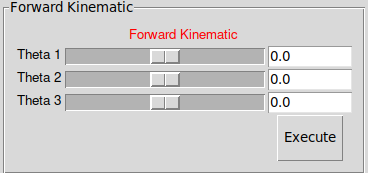
\includegraphics[width=1\linewidth]{Images/forw_ui.png}
	\caption{Giao diện Forward Kinematic}
	\label{fig:enter-label6}
\end{figure}

\subsubsection{Tạo animation và di chuyển robot theo bài toán động lực thuận}

Để tạo chuyển động cho robot ta sẽ lấy các giá trị góc $\theta$ mới trên UI và trừ đi góc $\theta$ hiện tại chia cho số bước ta muốn cho robot chuyển động sẽ ra được góc $\delta\theta$ cho mỗi bước di chuyển. Lưu tất cả các giá trị này vào một mảng các góc $\theta$ của robot sau mỗi bước di chuyển và tiến hành vẽ lại robot sau môi bước ta sẽ tạo được chuyển động cho robot.

\vspace{0.5cm}
\begin{lstlisting}[language=python]
	def forwardKine():
	deltaTime = 60
	nextTheta = np.array([guiTheta[0].get()*pi/180, guiTheta[1].get()*pi/180, guiTheta[2].get()*pi/180])
	stepAngle = np.array([(nextTheta[0]-theta[0])/deltaTime, (nextTheta[1]-theta[1])/deltaTime, (nextTheta[2]-theta[2])/deltaTime])
	animateTranform(nextTheta, stepAngle, deltaTime)
	
	def animateTranform(nextTheta, stepAngle, deltaTime):
	global animateArray, travelArray
	temp = np.array([0, 0, 0])
	for j in range(deltaTime):
	temp = temp+stepAngle
	animateArray = np.append(animateArray, theta+temp)
	animateArray = np.append(animateArray, nextTheta)
	animateArray = np.reshape(animateArray, (-1,3))
	travelArray = np.array([])
	
	def updateTheta():
	global theta, animateArray, travelArray
	if animateArray.size > 0:
	theta = animateArray[0]
	animateArray = animateArray[1:]
	T = updateTranposeMatrix()
	for i in range(2):
	guiCoor[i].set(coor2str(DHtranspose(baseO, T[i+2])))
	guiRPY.set(calRPY(T[3]))
	
	travelArray = np.append(travelArray, DHtranspose(baseO, T[3]))
	return T
\end{lstlisting}

\begin{figure}[H]
	\centering
	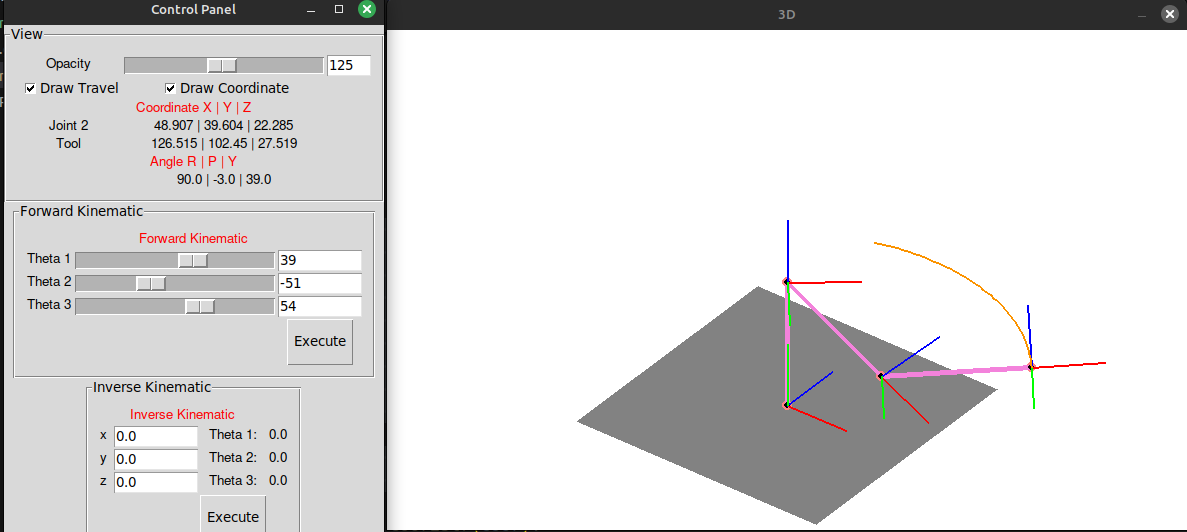
\includegraphics[width=1\linewidth]{Images/demo_forw.png}
	\caption{Forward Kinematic}
	\label{fig:enter-label7}
\end{figure}